% !TeX program = xelatex
\documentclass{beamer}
\usepackage{graphicx}
\usepackage{amsthm}
\usepackage{amsmath}
\usepackage{amssymb}
\usepackage{tikz,pgfplots}
\pgfplotsset{compat=1.18}
\usetikzlibrary{positioning, automata}
\usepackage{hyperref}
\usepackage{algorithm}
\usepackage{algpseudocode}

% Remove all \End commands  
\algnotext{EndIf}
\algnotext{EndFor}
\algnotext{EndWhile}
\algnotext{EndLoop}
\algnotext{EndForAll}
\algnotext{EndRepeat}
\algnotext{EndProcedure}
\algnotext{EndFunction}
\algnotext{Function}

\usepackage{tcolorbox}
\usepackage{xcolor} 
\usepackage{fontspec}
\usepackage{libertinus}
\usepackage[greek, english]{babel}
\usepackage{mathtools}
\usetikzlibrary{arrows,positioning, calc}
\tikzstyle{vertex}=[draw,fill=white,circle,minimum size=20pt,inner sep=0pt]
\usetikzlibrary{shapes.geometric, arrows}
\usepackage{listings}

\usetikzlibrary{shapes,decorations,decorations.pathreplacing,arrows,calc,arrows.meta,fit,positioning}

\tikzset{
    auto,node distance =1 cm and 1 cm, semithick,
    state/.style ={ellipse, draw, minimum width = 0.7 cm},
    point/.style = {circle, draw, inner sep=0.04cm,fill,node contents={}},
    bidirected/.style={Latex-Latex,dashed},
    directed/.style={-Latex},
    el/.style = {inner sep=2pt, align=left, sloped}
}

% Redefine Function command
\algdef{S}[FUNCTION]{Function}%
   [2]{\textproc{#1}\ifthenelse{\equal{#2}{}}{}{(#2)}}%

\algrenewcommand\alglinenumber[1]{\ifnum#1=0\else\footnotesize #1\fi}

% Define custom colors
\definecolor{myyellow}{RGB}{255,255,150}

% Define algorithmic environment inside a yellow-colored box
\newenvironment{yellowalgo}{
    \begin{tcolorbox}[colback=myyellow, colframe=myyellow, boxrule=0.5pt]
    \begin{algorithmic}[1]
    \setcounter{ALG@line}{-1}
}{
    \end{algorithmic}
    \end{tcolorbox}
}

% Custom command for function names
\newcommand{\Func}[1]{\textproc{#1}}

\renewcommand{\L}{\mathcal{L}}
\newcommand{\Create}{\textbf{Create} }
\DeclareMathOperator{\argmax}{argmax}
\DeclareMathOperator{\argmin}{argmin}
\newcommand{\True}{\texttt{True}}
\newcommand{\False}{\texttt{False}}

% ---- Beamer theme ----
\usetheme{Madrid}
\usecolortheme{default}
\setbeamertemplate{navigation symbols}{}



% Title info
\title{Συντομότερα Μονοπάτια}
\author[Α. Κολιόπουλος, Δ. Βογιατζής]{Αναστάσης Κολιόπουλος 22390104\\[0.2em] Δημήτρης Βογιατζής 22390015}
\date{}

\begin{document}

% ============ TITLE ============
\begin{frame}
\titlepage
\vfill
\begin{center}
    \includegraphics[width=0.25\textwidth]{UniWA logo.png}
\end{center}
\end{frame}

% ============================================================
%  ΕΙΣΑΓΩΓΗ
% ============================================================
\section{Εισαγωγή}

\begin{frame}{Βασικές Έννοιες}
\begin{itemize}
    \item Ένα \emph{κατευθυνόμενο γράφημα} $G = (V, E)$, με $|V|=n$, $|E|=m$.
    \item \emph{Ακμή} $e=(v,u) \in E$: ο $v$ προσπίπτει στον $u$.
    \item $N^+(v) = \{u : (v,u)\in E\}$, \quad $N^-(v) = \{u : (u,v)\in E\}$.
    \item \emph{Μονοπάτι}: ακολουθία κορυφών $\langle v_1,\dots,v_k\rangle$ χωρίς επαναλήψεις, με $v_{i+1}\in N^+(v_i)$.
    \item \emph{Κύκλος}: μονοπάτι με επαναλαμβανόμενες κορυφές.
    \item \emph{ΚΑΓ}: Κατευθυνόμενο Ακυκλικό Γράφημα.
\end{itemize}
\end{frame}

\begin{frame}{Συνάρτηση Βάρους \& Συντομότερο Μονοπάτι}
\begin{itemize}
    \item \emph{Συνάρτηση βάρους} $w : E \to \mathbb{R}$: κόστος μετακίνησης ανά ακμή.
    \item Θεωρούμε ότι δεν υπάρχει \emph{αρνητικός κύκλος}.
    \item Ένα \emph{συντομότερο μονοπάτι} $V_{\text{shortest}}$ ελαχιστοποιεί:
    \begin{align*}
        w(V_{\text{shortest}}) \leq w(V)
    \end{align*}
    για κάθε άλλο μονοπάτι $V$ με ίδια αφετηρία και τέλος.
    \item Στόχος: εύρεση του \textbf{κόστους} του συντομότερου μονοπατιού.
\end{itemize}
\end{frame}

% ============================================================
%  ΑΛΓΟΡΙΘΜΟΣ 1 — Συντομότερο μονοπάτι σε ΚΑΓ
% ============================================================
\section{Συντομότερο μονοπάτι σε ΚΑΓ}

\begin{frame}{Συντομότερο μονοπάτι σε ΚΑΓ --- Παρατήρηση}
\begin{block}{Παρατήρηση 1}
Έστω $V_{\text{shortest}} = \langle v_1,\dots,v_k\rangle$ ένα συντομότερο μονοπάτι από $s$ στη $v$.
Ορίζουμε $V^R_{\text{shortest}}$ με $v^R_i = v_{k-i+1}$ και $v^R_{i+1}\in N^-(v^R_i)$.
Αξιοποιούμε ότι:
\begin{equation*}
    \sum_{i=1}^{k-1} w(v_i,v_{i+1}) = \sum_{i=1}^{k-1} w(v^R_{i+1}, v^R_i).
\end{equation*}
\end{block}
\end{frame}

\begin{frame}{Συντομότερο μονοπάτι σε ΚΑΓ --- Επεξήγηση}
Αξιοποιούμε \emph{Δυναμικό Προγραμματισμό} στο ΚΑΓ:
\begin{itemize}
    \item $D(v)$: συντομότερο μονοπάτι από $v$ προς $s$.
    \item Αναδρομική σχέση:
    \begin{align*}
        d_v =
        \begin{cases}
            0, & v = s, \\
            \min_{u \in N^-(v)}\{d_u + w(u,v)\}, & v \neq s.
        \end{cases}
    \end{align*}
    \item Τα υποπροβλήματα λύνονται κατά \textbf{τοπολογική σειρά}.
    \item Πολυπλοκότητα: $\mathcal{O}(n + m)$.
\end{itemize}
\end{frame}

\begin{frame}{Συντομότερο μονοπάτι σε ΚΑΓ --- Κώδικας}
\begin{yellowalgo}
    \Function{Shortest-Path-in-DAG}{$G, s$}
        \For{\textbf{all} $v \in G.V \setminus \{s\}$}
            \State $D[v] \gets \infty;$
        \EndFor
        \State $D[s] \gets 0;$
        \State Διατάσσουμε τις κορυφές σε τοπολογική σειρά$;$
        \For{\textbf{all} $v \in G.V$}
            \For{\textbf{all} $u \in N^-(v)$}
                \If{$D[u] + w(u, v) < D[v]$}
                    \State $D[v] \gets D[u] + w(u, v);$
                \EndIf
            \EndFor
        \EndFor
        \State \Return $D;$
    \EndFunction
\end{yellowalgo}
\end{frame}

\begin{frame}{Συντομότερο μονοπάτι σε ΚΑΓ --- Σχήμα}
\begin{center}
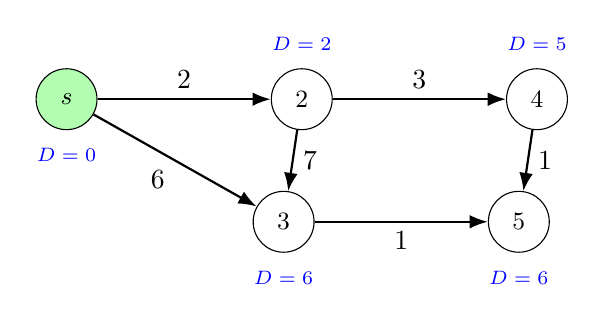
\begin{tikzpicture}[
    node distance=1.8cm and 2.2cm,
    vertex/.style={draw, circle, minimum size=22pt, inner sep=0pt, font=\small},
    edge label/.style={font=\scriptsize, auto},
    >=Latex
]
    % Nodes (topological order: s=1, 2, 3, 4, 5)
    \node[vertex, fill=green!30] (s) {$s$};
    \node[vertex, right=of s] (2) {$2$};
    \node[vertex, below right=1cm and 2.2cm of s] (3) {$3$};
    \node[vertex, right=of 2] (4) {$4$};
    \node[vertex, right=of 3] (5) {$5$};

    % Edges with weights
    \draw[->, thick] (s) -- node[above] {2} (2);
    \draw[->, thick] (s) -- node[below left] {6} (3);
    \draw[->, thick] (2) -- node[above] {3} (4);
    \draw[->, thick] (2) -- node[right] {7} (3);
    \draw[->, thick] (3) -- node[below] {1} (5);
    \draw[->, thick] (4) -- node[right] {1} (5);

    % Shortest path labels
    \node[below=3pt, font=\scriptsize, blue] at (s.south) {$D=0$};
    \node[above=3pt, font=\scriptsize, blue] at (2.north) {$D=2$};
    \node[below=3pt, font=\scriptsize, blue] at (3.south) {$D=6$};
    \node[above=3pt, font=\scriptsize, blue] at (4.north) {$D=5$};
    \node[below=3pt, font=\scriptsize, blue] at (5.south) {$D=6$};
\end{tikzpicture}
\end{center}
\vspace{0.3cm}
{\small Τοπολογική σειρά: $s \to 2 \to 3 \to 4 \to 5$.\\
Π.χ.\ $D[5] = \min\{D[3]+1,\; D[4]+1\} = \min\{7,\;6\} = 6$.}
\end{frame}

% ============================================================
%  ΑΛΓΟΡΙΘΜΟΣ 2 — DIJKSTRA
% ============================================================
\section{Αλγόριθμος Dijkstra}

\begin{frame}{Dijkstra --- Επεξήγηση}
\begin{itemize}
    \item Εφαρμόζεται σε γραφήματα με \textbf{μη αρνητικά} βάρη (όχι απαραίτητα ΚΑΓ).
    \item Σε κάθε επανάληψη:
    \begin{enumerate}
        \item Επιλέγει την κορυφή $v$ με ελάχιστο $D[v]$ από τις μη οριστικοποιημένες.
        \item \emph{Οριστικοποιεί} τη $v$ (τελική απόσταση).
        \item \emph{Χαλαρώνει} τις ακμές που εκκινούν από τη $v$.
    \end{enumerate}
    \item Πολυπλοκότητα:
    \begin{itemize}
        \item Σωρός Fibonacci: $\Theta(n \lg n + m)$
        \item Δυαδικός σωρός: $\Theta((n+m)\lg n)$
    \end{itemize}
\end{itemize}
\end{frame}

\begin{frame}{Dijkstra --- Κώδικας}
\begin{yellowalgo}
\Function{Dijkstra}{$G, s$}
    \For{\textbf{all} $v \in G.V \setminus \{s\}$}
        \State $D[v] \gets \infty;$
    \EndFor
    \State $D[s] \gets 0;$
    \State $S \gets \emptyset;$
    \While{$S \neq G.V$}
        \State $v \gets {\arg\min}\{D[u] : u \in G.V \setminus S\};$
        \State $S \gets S \cup \{v\};$
        \For{\textbf{all} $u \in N^+(v) \setminus S$}
            \If{$D[v] + w(v, u) < D[u]$}
                \State $D[u] \gets D[v] + w(v, u);$
            \EndIf
        \EndFor
    \EndWhile
    \State \Return $D;$
\EndFunction
\end{yellowalgo}
\end{frame}

\begin{frame}{Dijkstra --- Σχήμα}
\begin{center}
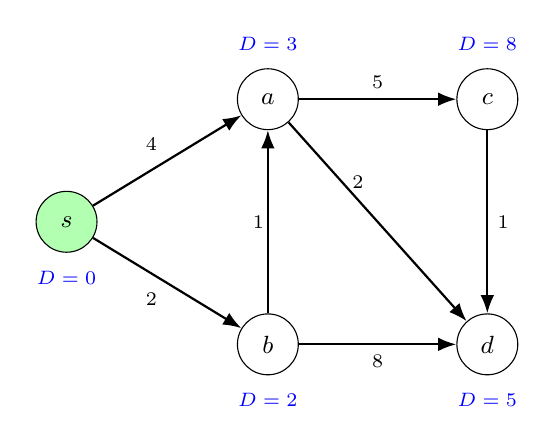
\begin{tikzpicture}[
    vertex/.style={draw, circle, minimum size=22pt, inner sep=0pt, font=\small},
    >=Latex, node distance=2cm
]
    \node[vertex, fill=green!30] (s) {$s$};
    \node[vertex, above right=1cm and 2cm of s] (a) {$a$};
    \node[vertex, below right=1cm and 2cm of s] (b) {$b$};
    \node[vertex, right=2cm of a] (c) {$c$};
    \node[vertex, right=2cm of b] (d) {$d$};

    \draw[->, thick] (s) -- node[above left, font=\scriptsize] {4} (a);
    \draw[->, thick] (s) -- node[below left, font=\scriptsize] {2} (b);
    \draw[->, thick] (a) -- node[above, font=\scriptsize] {5} (c);
    \draw[->, thick] (b) -- node[left, font=\scriptsize, fill=white, inner sep=1pt, pos=0.5] {1} (a);
    \draw[->, thick] (b) -- node[below, font=\scriptsize] {8} (d);
    \draw[->, thick] (a) -- node[right, font=\scriptsize, pos=0.3] {2} (d);
    \draw[->, thick] (c) -- node[right, font=\scriptsize] {1} (d);

    \node[below=3pt, font=\scriptsize, blue] at (s.south) {$D=0$};
    \node[above=3pt, font=\scriptsize, blue] at (a.north) {$D=3$};
    \node[below=3pt, font=\scriptsize, blue] at (b.south) {$D=2$};
    \node[above=3pt, font=\scriptsize, blue] at (c.north) {$D=8$};
    \node[below=3pt, font=\scriptsize, blue] at (d.south) {$D=5$};
\end{tikzpicture}
\end{center}
\vspace{0.2cm}
{\small Σειρά οριστικοποίησης: $s\;(0) \to b\;(2) \to a\;(3) \to d\;(5) \to c\;(8)$.\\
Π.χ.\ $D[a] = \min\{4,\; 2+1\} = 3$ μετά χαλάρωση από $b$.}
\end{frame}

% ============================================================
%  ΑΛΓΟΡΙΘΜΟΣ 3 — BELLMAN-FORD
% ============================================================
\section{Αλγόριθμος Bellman-Ford}

\begin{frame}{Bellman-Ford --- Παρατήρηση}
\begin{block}{Παρατήρηση 2}
Ένα συντομότερο μονοπάτι περιέχει το πολύ $n - 1$ ακμές.
\end{block}
\vspace{0.5cm}
\begin{itemize}
    \item Αν ένα μονοπάτι είχε $\geq n$ κορυφές, θα περιείχε κύκλο.
    \item Ο κύκλος αυτός δεν μπορεί να είναι αρνητικός (υπόθεση).
    \item Άρα μπορούμε να τον αφαιρέσουμε χωρίς αύξηση κόστους.
\end{itemize}
\end{frame}

\begin{frame}{Bellman-Ford --- Επεξήγηση}
Εφαρμόζεται σε γραφήματα με \textbf{αρνητικά βάρη} (χωρίς αρνητικό κύκλο).
\begin{itemize}
    \item $D(i, v)$: συντομότερο μονοπάτι από $v$ στο $s$ με $\leq i$ ακμές.
    \item Αναδρομική σχέση:
    \begin{align*}
        d_{i,v} =
        \begin{cases}
            0, & i=0,\; v=s, \\
            \infty, & i=0,\; v \neq s, \\
            \min\{d_{i-1,v},\;\min_{u\in N^-(v)}\{d_{i-1,u}+w(u,v)\}\}, & i\geq 1.
        \end{cases}
    \end{align*}
    \item Υποπροβλήματα: αύξουσα σειρά $i$.
    \item Πολυπλοκότητα: $\mathcal{O}(n \cdot m)$.
\end{itemize}
\end{frame}

\begin{frame}{Bellman-Ford --- Κώδικας}
\begin{yellowalgo}
    \Function{Bellman-Ford}{$G, s$}
        \For{\textbf{all} $v \in G.V \setminus \{s\}$}
            \State $D[0][v] \gets \infty;$
        \EndFor
        \State $D[0][s] \gets 0;$
        \For{$i \gets 1; \; i \leq n - 1; \; i++$}
            \For{\textbf{all} $v \in G.V$}
                \State $D[i][v] \gets D[i - 1][v];$
                \For{\textbf{all} $u \in N^-(v)$}
                    \State $D[i][v] \gets \min\{D[i][v], D[i-1][u] + w(u,v)\};$
                \EndFor
            \EndFor
        \EndFor
        \State \Return $D;$
    \EndFunction
\end{yellowalgo}
\end{frame}

\begin{frame}{Bellman-Ford --- Σχήμα}
\begin{center}
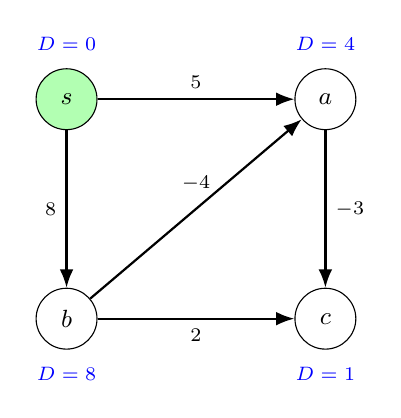
\begin{tikzpicture}[
    vertex/.style={draw, circle, minimum size=22pt, inner sep=0pt, font=\small},
    >=Latex, node distance=2cm
]
    \node[vertex, fill=green!30] (s) {$s$};
    \node[vertex, right=2.5cm of s] (a) {$a$};
    \node[vertex, below=2cm of s] (b) {$b$};
    \node[vertex, right=2.5cm of b] (c) {$c$};

    \draw[->, thick] (s) -- node[above, font=\scriptsize] {5} (a);
    \draw[->, thick] (s) -- node[left, font=\scriptsize] {8} (b);
    \draw[->, thick] (a) -- node[right, font=\scriptsize] {$-3$} (c);
    \draw[->, thick] (b) -- node[below, font=\scriptsize] {2} (c);
    \draw[->, thick] (b) -- node[above, font=\scriptsize, pos=0.5, yshift=3pt] {$-4$} (a);

    \node[above=3pt, font=\scriptsize, blue] at (s.north) {$D=0$};
    \node[above=3pt, font=\scriptsize, blue] at (a.north) {$D=4$};
    \node[below=3pt, font=\scriptsize, blue] at (b.south) {$D=8$};
    \node[below=3pt, font=\scriptsize, blue] at (c.south) {$D=1$};
\end{tikzpicture}
\end{center}
\vspace{0.2cm}
{\small
\begin{tabular}{c|cccc}
     & $s$ & $a$ & $b$ & $c$ \\ \hline
    $i=0$ & 0 & $\infty$ & $\infty$ & $\infty$ \\
    $i=1$ & 0 & 5 & 8 & $\infty$ \\
    $i=2$ & 0 & 4 & 8 & 2 \\
    $i=3$ & 0 & 4 & 8 & 1 \\
\end{tabular}
\quad Π.χ.\ $D[2][a] = \min\{5,\; 8+(-4)\} = 4$.
}
\end{frame}

% ============================================================
%  ΑΛΓΟΡΙΘΜΟΣ 4 — FLOYD-WARSHALL
% ============================================================
\section{Αλγόριθμος Floyd-Warshall}

\begin{frame}{Floyd-Warshall --- Επεξήγηση}
Βρίσκει συντομότερα μονοπάτια για \textbf{όλα τα ζεύγη} κορυφών.
\begin{itemize}
    \item $D(i,v,u)$: συντομότερο μονοπάτι $v \to u$ περνώντας από κορυφές $\{1,\dots,i\}$.
    \item Αναδρομική σχέση:
    \begin{align*}
        d_{i,v,u} =
        \begin{cases}
            0, & i=0,\; v=u, \\
            w(v,u), & i=0,\; (v,u)\in E, \\
            \infty, & i=0,\; (v,u)\notin E, \\
            \min\{d_{i-1,v,u},\; d_{i-1,v,i}+d_{i-1,i,u}\}, & i\geq 1.
        \end{cases}
    \end{align*}
    \item Πολυπλοκότητα: $\mathcal{O}(n^3)$.
\end{itemize}
\end{frame}

\begin{frame}{Floyd-Warshall --- Κώδικας}
\begin{yellowalgo}
    \Function{Floyd-Warshall}{$G$}
        \For{\textbf{all} $v \in G.V$}
            \State $D[0][v][v] \gets 0;$
            \For{\textbf{all} $u \in G.V \setminus \{v\}$}
                \If{$(v, u) \in G.E$}
                    \State $D[0][v][u] \gets w(v, u);$
                \Else     
                    \State $D[0][v][u] \gets \infty;$
                \EndIf
            \EndFor
        \EndFor
        \For{$i \gets 1; \; i \leq n; \; i++$}
            \For{\textbf{all} $v \in G.V$}
                \For{\textbf{all} $u \in G.V$}
                    \State $D[i][v][u] \gets \min\{D[i-1][v][u],\; D[i-1][v][i]+D[i-1][i][u]\};$
                \EndFor
            \EndFor
        \EndFor
        \State \Return $D;$
    \EndFunction
\end{yellowalgo}
\end{frame}

\begin{frame}{Floyd-Warshall --- Σχήμα}
\begin{center}
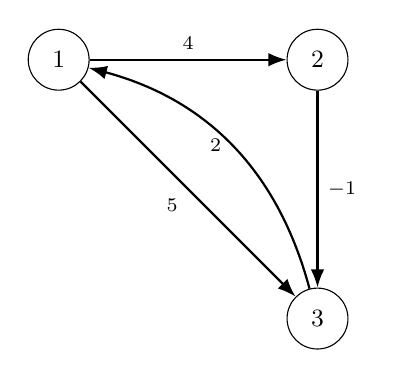
\begin{tikzpicture}[
    vertex/.style={draw, circle, minimum size=22pt, inner sep=0pt, font=\small},
    >=Latex, node distance=2.5cm
]
    \node[vertex] (1) {$1$};
    \node[vertex, right=of 1] (2) {$2$};
    \node[vertex, below=of 2] (3) {$3$};

    \draw[->, thick] (1) -- node[above, font=\scriptsize] {4} (2);
    \draw[->, thick] (2) -- node[right, font=\scriptsize] {$-1$} (3);
    \draw[->, thick] (1) -- node[below left, font=\scriptsize] {5} (3);
    \draw[->, thick] (3) to[bend right=30] node[left, font=\scriptsize] {2} (1);
\end{tikzpicture}
\end{center}
\vspace{0.2cm}
{\small
$D^{(0)}$: αρχικά βάρη ακμών.\quad
$D^{(1)}$: ενδιάμεσος $\{1\}$.\quad
$D^{(2)}$: ενδιάμεσοι $\{1,2\}$.\quad
$D^{(3)}$: τελικό.

\vspace{0.2cm}
\begin{tabular}{c|ccc}
$D^{(3)}$ & 1 & 2 & 3 \\ \hline
1 & 0 & 4 & 3 \\
2 & 1 & 0 & $-1$ \\
3 & 2 & 6 & 0 \\
\end{tabular}
\quad Π.χ.\ $d_{3,1,3} = \min\{5,\; 4+(-1)\} = 3$ (μέσω κορυφής 2).
}
\end{frame}

% ============ BIBLIOGRAPHY ============

\begin{frame}{Βιβλιογραφία}
\begin{thebibliography}{99}
\bibitem{dmagos}
Δημήτριος Μάγος.
\textit{Στοιχεία Ανάλυσης Αλγορίθμων}.
Εκδόσεις Τσότρας, 2024.

\bibitem{tsichlas}
Τσίχλας, Κ., Γούναρης, Α., Μανωλόπουλος, Ι. (2015). \textit{Σχεδίαση και Ανάλυση Αλγορίθμων}. Κάλλιπος.

\bibitem{cormen2022}
Cormen, Leiserson, Rivest, Stein.
\textit{Introduction to Algorithms}. 4η Έκδοση, MIT Press, 2022.

\bibitem{levitin2022}
Anany Levitin.
\textit{Introduction to the Design and Analysis of Algorithms}. 4η Έκδοση, Pearson, 2022.
\end{thebibliography}
\end{frame}

\end{document}
